\documentclass[10pt,conference,compsocconf]{IEEEtran}

\usepackage{hyperref}
\usepackage{graphicx}	% For figure environment
\usepackage{subcaption}
\usepackage{amsmath}
\usepackage{bm}
\usepackage{tikz}
\usepackage{tikz-qtree}
\usepackage{amsmath}
\usepackage{amssymb}
\usepackage{amsfonts}
\usepackage{amsthm}
\usepackage{mathrsfs}
\usepackage{cleveref}
\usepackage{xcolor}
\usepackage{nicefrac}
\usepackage{graphicx}
\usepackage{subcaption}
\usepackage{mwe}
\usetikzlibrary{trees,calc,arrows.meta,positioning,decorations.pathreplacing,bending}


\begin{document}
\title{Deep Learning --- Miniproject 2}

\author{
  Olesia Altunina (285467), Mauro Pfister (235440), Joey Zenhaeusern (226652)
}

\maketitle

\section{Introduction}
The goal of this project was to implement a neural network to tackle a specific binary classification problem and assess the performance improvement achieved by employing weight sharing or/and auxiliary losses. The task was, given an ordered pair of MNIST samples, to predict whether the first digit is less or equal to the second.

\section{Networks}
To test the performance due to different architectures, we tried three basic network types. The first one, \texttt{BasicNet1}, is an ordinary CNN (CNN “feature detector” + MLP “classifier”) that takes a \textit{2 x 14 x 14} tensor as an input and makes predictions solely based on the binary targets. The second one, \texttt{AuxNet1}, is a CNN with weight sharing and auxiliary losses that make use of the digit classes available. The inputs, two separate \textit{1 x 14 x 14} tensors, are fed into the CNN + MLP to make digit predictions, which are then concatenated into a single vector and fed into the binary classifier (another MLP). Finally, the last architecture that we used, is implemented in the \texttt{AuxNet2} class. This constitutes an Inception-like architecture that takes in two separate tensors, runs them through a “feature detector” (CNN), and then branches the outputs into two classifiers, one for digit recognition, the other for binary classification.
\texttt{AuxNet3} is similar to \texttt{AuxNet2} but has 2 convolutional and 3 linear layers (vs 3 conv and 2 linear layers for the previous models). This one was built to check how the distribution of layers might influence the performance.

In the last two architectures, the loss is cumulative of the three losses: the losses of the first and second digit recognition and the binary classification loss.

We used cross-entropy losses due to classification character of the problem, Adam optimiser as the one that converges the fastest with less parameter tuning, and 0.5 dropout on all linear layers for regularisation.

\section{Training and Optimisation}
\subsection{Implementation}
\texttt{Model} is the child class of \texttt{torch.nn.Module} that allows to perform the training of multiple runs of the same network with different parameters, in this particular case the following:
\begin{itemize}
    \item \textbf{Network parameters} such as the number of channels for convolutional layers and the number of hidden units for linear layers,
    \item \textbf{Learning rate},
    \item \textbf{Batch size}.
\end{itemize}
Running \textit{src/test.py} with no arguments reproduces the training of the fastest sufficient model. When adding \texttt{--train\_best} argument, it trains the best model (takes longer). When adding \texttt{--reproduce\_all} argument, it reproduces the complete process of training and optimisation.

\subsection{Optimisation Protocol}
To optimise the network parameters, we generated for each net a list of all possible combinations of sizes with values in {16, 32, 64, 128, 256, 512} that yielded the number of trainable parameters between 65000 and 75000. For each of these sets of parameters, we trained the corresponding nets 5 times. The learning rate was fixed at 0.005 and the batch size at 100.

To optimise the learning rate and the batch size, we picked the best model with the best mean validation accuracy and varied learning rate in {0.0001, 0.0005, 0.001, 0.005, 0.01} with the fixed batch size of 100, and batch sizes in {25, 50, 100, 200, 500, 1000} with the fixed learning rate of 0.005.

\section{Results}
The network parameters for the 4 described nets can be found in Fig. 1. The discrepancy in mean validation accuracy is between ~58\% and ~94\%. It is worth noticing that among the best results there are the models with varying convolutional layers sizes (32-128-64, 128-32-64), and that the lower the accuracy, generally the more the variance of the sample. Among the 4 models, the best is AuxNet2, AuxNet3 being ~5\% behind, which suggests that having more convolutional layers, and not linear ones, may be advantageous.

The best learning rate and batch size are shown in Fig. 2.

\section{Conclusion}
Indeed, shared weights and auxiliary losses are helpful for the tasks where the decision is made based on a few separate inputs. But an ordinary CNN with the inputs stacked as channels and with no auxiliary losses also performs better than naive, implying that there are some shared patterns that a CNN can discriminate.

\pagebreak

\begin{figure*}
    \centering
    \begin{subfigure}[b]{0.475\textwidth}
        \centering
        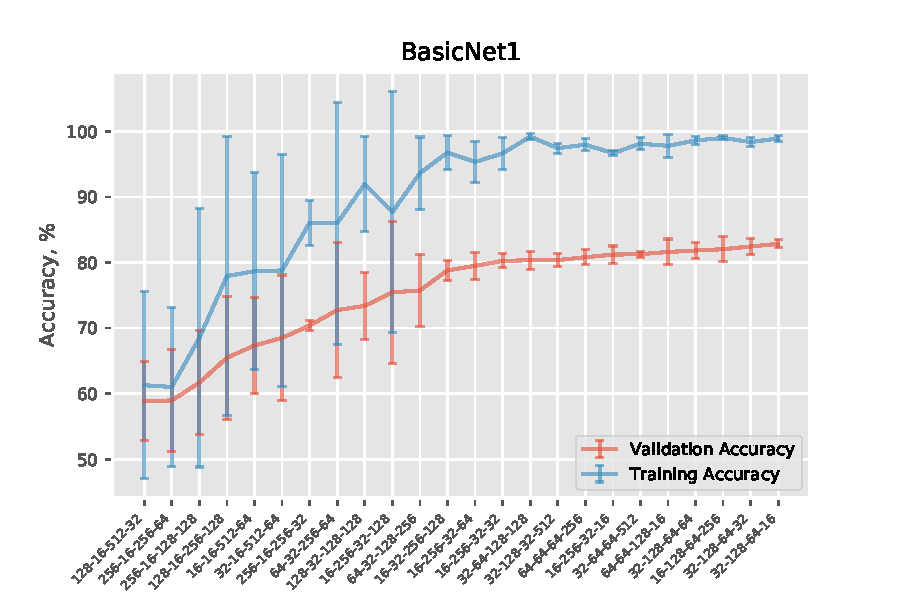
\includegraphics[width=\textwidth]{BasicNet1.pdf}
        \label{fig:BasicNet1}
    \end{subfigure}
    \hfill
    \begin{subfigure}[b]{0.475\textwidth}  
        \centering 
        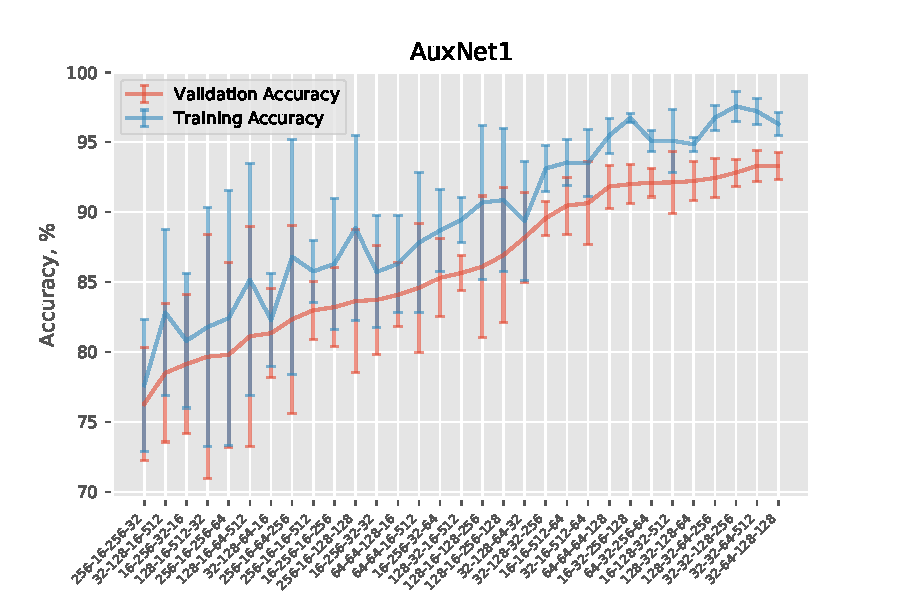
\includegraphics[width=\textwidth]{AuxNet1.pdf}
        \label{fig:AuxNet1}
    \end{subfigure}
    \vskip\baselineskip
    \begin{subfigure}[b]{0.475\textwidth}   
        \centering 
        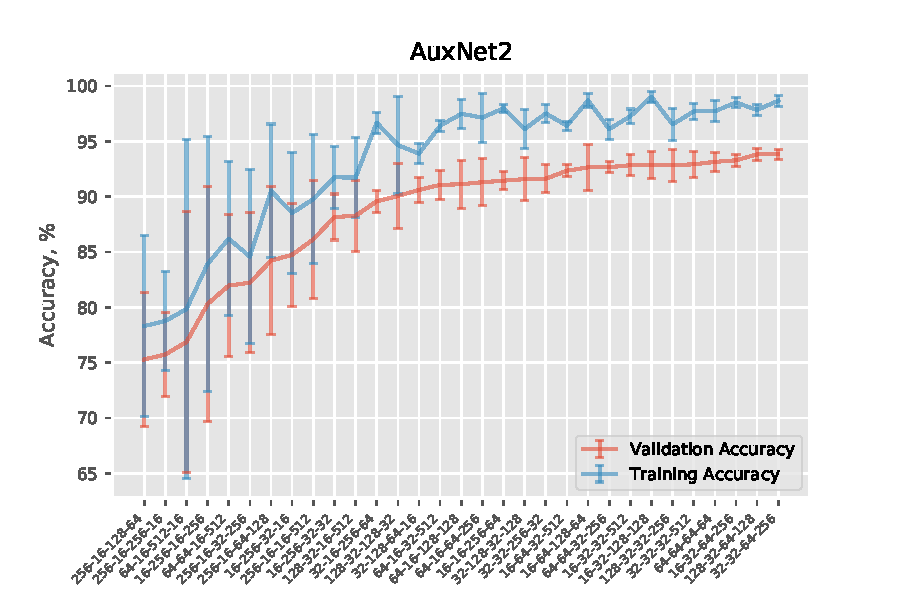
\includegraphics[width=\textwidth]{AuxNet2.pdf}
        \label{fig:AuxNet2}
    \end{subfigure}
    \quad
    \begin{subfigure}[b]{0.475\textwidth}   
        \centering 
        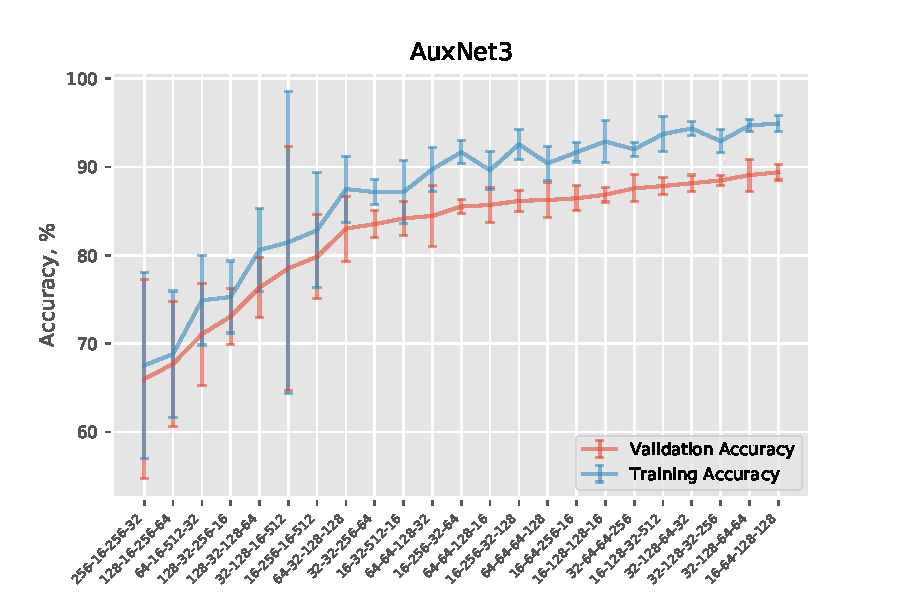
\includegraphics[width=\textwidth]{AuxNet3.pdf}
        \label{fig:AuxNet3}
    \end{subfigure}
    \caption[ Best accuracy and the network parameters. ]
    {\small Best accuracy vs the network parameters.} 
    \label{fig:mean and std of nets}
\end{figure*}

\begin{figure*}
    \centering
    \begin{subfigure}[b]{0.475\textwidth}
        \centering
        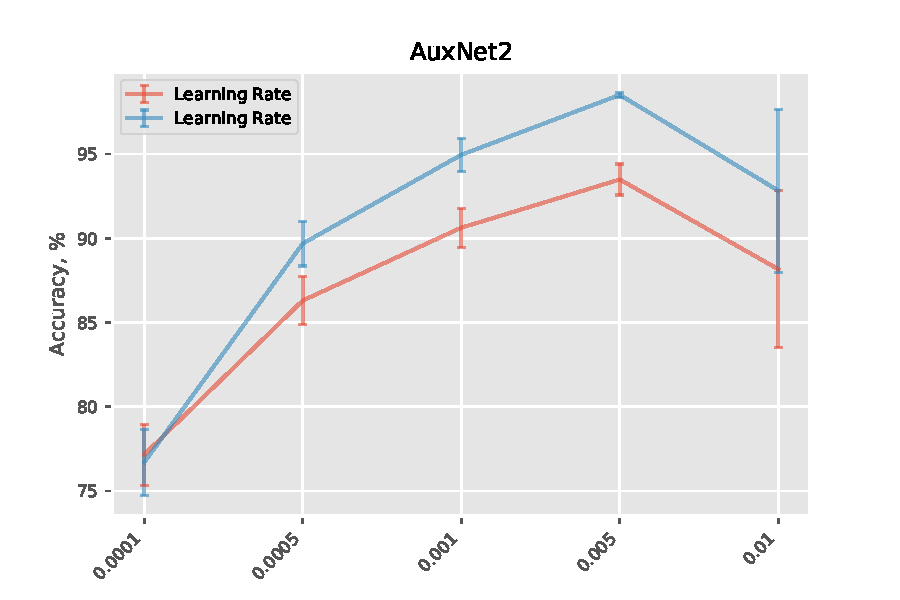
\includegraphics[width=\textwidth]{learning_rates.pdf}
        \label{fig:learning_rates}
    \end{subfigure}
    \hfill
    \begin{subfigure}[b]{0.475\textwidth}  
        \centering 
        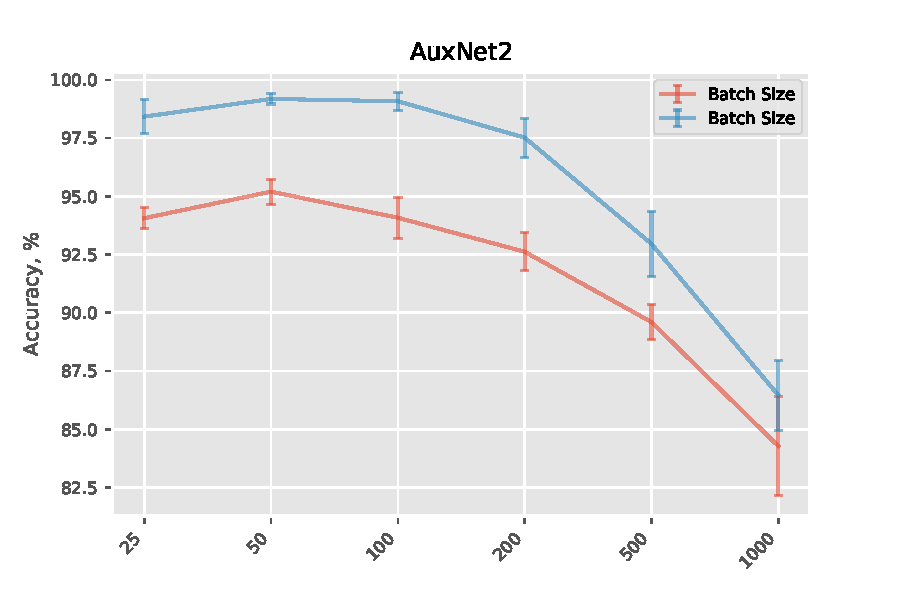
\includegraphics[width=\textwidth]{batch_sizes.pdf}
        \label{fig:batch_sizes}
    \end{subfigure}
    \caption[ Best learning rate and batch size. ]
    {\small Best learning rate and batch size.} 
    \label{fig:mean and std of nets}
\end{figure*}

\bibliographystyle{IEEEtran}
\bibliography{literature}

\end{document}